\documentclass[11pt,a4paper]{article}

\usepackage{CJKutf8}
\usepackage[T1]{fontenc}
\usepackage[utf8]{inputenc}
\usepackage[]{tikz}
%\usetikzlibrary{graphdrawing}
%\usepackage{ucs}
\usepackage{amsthm} %numéroter les questions
\usepackage[frenchb]{babel}
\usepackage{datetime}
\usepackage{xspace} % typographie IN
\usepackage{hyperref}% hyperliens
\usepackage[all]{hypcap} %lien pointe en haut des figures
\usepackage[french]{varioref} %voir x p y
\usepackage{fancyhdr}% en têtes
%\input cyracc.def
\usepackage{pgfplots}
\usetikzlibrary{babel,positioning,calc}
\usepackage[]{graphicx} %include pictures
\usepackage[siunitx ]{circuitikz}
\usepackage{gnuplottex}
\usepackage{ifthen}

\usepackage[top=1.3 in, bottom=1.3 in, left=1.3 in, right=1.3 in]{geometry} % Yeah, that's bad to play with margins
\usepackage[]{pdfpages}

\usepackage[]{attachfile}

\newdateformat{mydate}{2016--2017}%hack pour remplacer \THEYEAR

%cyr
\newcommand\textcyr[1]{{\fontencoding{OT2}\fontfamily{wncyr}\selectfont #1}}

\input{stegano.tex}

\newboolean{corrige}
\setboolean{corrige}{true}%corrigé
%\setboolean{corrige}{false}% pas de corrigé

\newboolean{annexes}
\setboolean{annexes}{true}%annexes
%\setboolean{annexes}{false}% pas de annexes

\newboolean{mos}
%\setboolean{mos}{true}%annexes
\setboolean{mos}{false}% pas de annexes

\usepackage{aeguill} %guillemets

%\usepackage{CJK} %Chinese 

%\usetikzlibrary{graphs} 
\usetikzlibrary{graphs}

%\setCJKmainfont{SimSun}

%% fancy header & foot
\pagestyle{fancy}
\lhead{[ELEC-H-301] Électronique appliquée\\ Labo \no 4 : ampli à transistors}
\rhead{\mydate\today\\ page \thepage}
\chead{\ifthenelse{\boolean{corrige}}{Corrigé}{}}
\cfoot{}
%%

\pdfinfo{
/Author (Yannick Allard, ULB -- BEAMS)
/Title (Labo 4 ELEC-H-301, transistor MOS)
/ModDate (D:\pdfdate)
}

\hypersetup{
pdftitle={Labo 4 [ELEC-H-301] Électronique appliquée : ampli à transistors},
pdfauthor={Yannick Allard, ©2010-2016 ULB - BEAMS  },
pdfsubject={Transistor MOS en amplification}
}

\theoremstyle{definition}% questions pas en italique
\newtheorem{Q}{Question}[] % numéroter les questions [section] ou non []

\newcommand{\reponse}[1]{% pour intégrer une réponse : \reponse{texte} : sera inclus si \boolean{corrige}
	\ifthenelse {\boolean{corrige}} {\paragraph{Réponse :} #1} {}
 }

\newcommand{\addcontentslinenono}[4]{\addtocontents{#1}{\protect\contentsline{#2}{#3}{#4}{}}}

\date{\vspace{-1cm}\mydate\today}
\title{\vspace{-2cm} Labo \no 4\\ Électronique appliquée [ELEC-H-301]\\Réalisation d'un ampli à transistor\ifthenelse{\boolean{corrige}}{~\\Corrigé}{}}

%\author{\vspace{-1cm}}%\textsc{Yannick Allard}}

\setlength{\parskip}{0.5cm plus4mm minus3mm} %espacement entre §
\setlength{\parindent}{0pt}

\begin{document}

%
\section{Synthèse -- dimensionnement d'un étage}

\textit{Cahier des charges :}
\begin{itemize}
\item Bande passante : 20Hz--20kHz
\item Gain : 26dB
\item Am\pl{``Giving up something that no longer serves a purpose, or protects you, or
helps you, isn’t giving up at all, it’s growing up."}{Laurell K. Hamilton}litude de l'entrée : 0.1V, sinusoïdale, moyenne nulle
\item Tension de sortie à moyenne nulle
\item Impédance d'entrée : $Z_{in}\geq10k\Omega$
\item Impédance de sortie : $Z_{out}\leq 1k\Omega$
\item Puissance statique dissipée par le transistor : $P_T\leq 0.5W$
\item Alimentation : $12V$ continue
\item Impédance de la charge : $Z_{ch}\geq 3.3k\Omega$
\end{itemize}


~\\
\textit{Démarche proposée :}
\begin{enumerate}
\item Identifier les contraintes im\pl{``The one who finds you drowning in shallow water and simply helps you out
without commenting on the depth of the water is a rare gift."}{Shabaz Khan}osées par le cahier des charges\dl{Li \& Summer, thank you for the quotes :-)}{}
\item Choisir la topologie de l'amplificateur (= schéma que vous avez obtenu en répondant aux questions du labo).
\item Identifier les différents \pl{``A person who feels appreciated will always do more than what is expected."}{Amy Rees Anderson}aramètres en fonction du cahier des charges (faire un schéma à petit signal).
\item Dimensionner les valeurs des différents composants du circuit sur base des courbes théoriques en annexe.
\item Déterminer la valeur de la tension de polarisation.
\item {Vérifier expérimentalement}\footnote{Ce point ne sera pas abordé dans ce document.} en tenant compte des caractéristiques réelles de votre transistor. La polarisation devra être ajustée pour obtenir le bon gain\dl{``Please, calm down and breathe."}{Queena}
%\item 
\end{enumerate}

{\color{white}C'est parti ! On se motive et on y va, tout va bien se passer !}

\begin{center}
\begin{CJK}{UTF8}{gbsn}
破釜沉舟,百二秦关终属楚\\
卧薪尝胆,三千越甲可吞吴\\
祝你考试成功!\\
考试必过,加油!
\end{CJK}

\end{center}



%\begin{Q}
%\vspace{-0.3cm}
%\begin{enumerate}
%\item Sur base des courbes fournies en annexe du labo, dimensionner un étage amplificateur ayant un gain de $26dB$ pour un signal d'entrée d'amplitude $0.1V$. L'impédance de charge du montage sera supérieure à $3.3k\Omega$. Le montage doit consommer moins de $0.5W$. 
%\item Vérifier expérimentalement en tenant compte des caractéristiques réelles de votre transistor. \textbf{Cette partie ne sera pas abordée dans ce document.}

%\end{enumerate}

\reponse{
~\\
%\appendix
%\section{dimensionnement}
\subsection{Contraintes :}
\begin{enumerate}
\item Gain de $26dB$ $\Longrightarrow$ $A_v= \pm 20$
\item Tension d'entrée (amplitude) : $V_{in}=0.1V$ $\Longrightarrow$ $V_{out}=2V$, moyennes nulles
\item $Z_{ch}\geq 3.3k\Omega$, $Z_{in}\geq10k\Omega$, $Z_{out}\leq 1k\Omega$
\item $E=12V$
\item $P_T=P_{\mbox{transistor}}\leq 0.5W$ il s'agit de la puissance statique dissipée par le transistor (et uniquement par le transistor)
\item $BW=20 \rightarrow 20kHz$
%\item Entrée et sortie à moyennes nulles
\end{enumerate}

\subsection{Topologie :}

On utilise le schéma de l'amplificateur inverseur à NMOS (inverseur) du labo :
\begin{center}
			%\includegraphics[width=8cm]{}
			\begin{circuitikz}[scale=1]\draw
			(0,1) to [short,o-] (9,1)
			(4,6) to [short] (9,6)
			(0,3) node[anchor=east] {In} to [short,o-] (1,3)
			(0,3) to [open, v_=$V_{in}$]  (0,1)
			(1,3) to [C=$C_{in}$ ](1.5,3)
			(1.5,3) to [short,-*] (2,3)
	%
			(2,6) node[alimp ] (alim) {}
			(alim.text) node {$+V_{dc}$}
	%		
			(2,3) to [R, l_=$R_{b1}$](2,6)
			(2,3) to [R=$R_{b2}$](2,1)
	%		
			(4,3) node[nigfetec] (mos) {}
			%(mos.B) node[anchor=west] {B}
			(mos.G) to [short] (2,3)
	%		
			(mos.D) to (4,4) to [R, l_=$R_D$] (4, 6)		
			%(4,5.5) to [R] (mos.D)
	%		
			(mos.D) to [short,-*](4,3.5)  to [short] (4.25,3.5)
	%		
			(mos.S) to [short] (4,1)% to [short, -o](2,0)  node[anchor=west] {S}
	%		
			(4.25,3.5) to [C, l^=$C{out}$] (6,3.5) to  [short](6,3.5) to [short,-o](6.5,3.5)node [anchor=south] {Out}	
			(6,3.5) to [generic, l_=$Z_{ch}$] (6,1)
			(6.5,3.5) to [open,v^=$V_{out}$] (6.5,1)
	%		
			(9,1) to [battery, l_=$E$](9,6)
	%		%(1,0) to [short, -o](-1,0)  node[anchor=east] {S}
	%		
	%%			(0,0) node[anchor=east] {In} 
	%%			to [short, o-] (1,0) 
	%%			to [open, v=$V_{GS}$] (1,-2)
	%%			to [short, -o] (0,-2)
	%%			to  (0,-2) node[anchor=east] {S}
	%%			to [short] (3,-2)
	%%			(3,0) to [cI=$ g_m \cdot V_{GS}$] (3,-2)
	%%			(3,-2) to [short, -o] (4,-2) node[anchor=west] {S}
	%%			(3,0) to [short, -o] (4,0)
	%%			to node[anchor=west] {D} (4,0)
	%	%		
			;\end{circuitikz}
	\end{center}
	
	Cette topologie impose que $Av=-20$ car cet étage d'amplification est inverseur.

%\subsection{Paramètres}

\subsection{Dimensionnement du gain et du point de polarisation}
Processus:
\begin{enumerate}
\item Dimensionnement du gain à vide
\item Choix d'un point de polarisation
\item Influence de la charge sur le gain
\end{enumerate}

On connaît le gain de cet étage\textbf{ à vide }lorsqu'il est polarisé correctement, il suffit d'analyser le schéma équivalent à petits signaux (voir labo) :

$$V_{out}=-g_m\cdot  R_D \cdot V_{in}$$

d'où : $$A_v=-g_m\cdot  R_D =-20$$

%L'influence de la charge sera étudiée à la fin de cette partie.

La limite en puissance $P_T=\frac{E}{2}\cdot I_D\leq0.5W$ (\textit{cf} Q.1 du labo) impose $I_D\leq 83mA$ avec $E=12V$. (Attention : seule la consommation statique du transistor est prise en compte ici)

On obtient alors $g_m\leq0.21S$ pour $I_D\leq83mA$ (voir courbes).

En pratique, on peut imposer $I_D$, $g_m$ ou $R_D$, mais il faut veiller à ce que la charge ait une faible influence sur le gain ($R_{D}\ll R_{ch}$). Pour un même gain, il est donc intéressant de choisir $R_D$ la plus faible possible, ce qui implique que $g_m$ sera plus grand et donc $I_D$ également. Le choix de $I_D$ n'est plus contraint que par la puissance dissipée par le transistor (et également le gain).

Si on impose $I_D=40mA<83mA$, $g_m=0.162S$ (voir courbes).

Alors on a $R_D=125\Omega$. En prenant la valeur normalisée la plus proche ($150\Omega$), on obtient $V_{DS}=6V$. % (la contrainte d'excursion de sortie de $2V$ minimum est respectée).
(L'influence de la charge a été négligée dans un premier temps)

$V_{GS}=2.95V$ d'où $V_{dc}=5.9V$ avec $R_{b1}=R_{b2}$.

En traçant la droite de charge sur le graphe $I_D=f\left(V_{DS}\right)$, on peut déterminer que l'amplitude maximum du signal de sortie vaut $\approx 5.5V$ ($>2V$ nécessaires).

Il faut vérifier que l'influence de la charge reste faible sur le gain : $R_D\ll R_{ch}$ permet de négliger $R_{ch}$ dans l'expression complète du gain $A_v=-g_m\cdot \left( R_D//R_{ch} \right)$ dans la bande passante du montage.

Le choix de $R_D=150\Omega$ implique une imprécision de $\approx 16\%$ sur le gain. %Il ne faut pas oublier que le $g_m$ est donné avec une dispersion de 100\%
Cette imprécision sera corrigée en pratique par un étalonnage du montage (qui restera très sensible à la température de toute façon).

\begin{center}
\fbox{$E=12V$}
\fbox{$R_D=150\Omega$}
\fbox{$I_D=40mA$}
\fbox{$P_T=240mW$}
\fbox{$V_{dc}=5.9V$}
\fbox{$R_{b1}=R_{b2}$}
\end{center}
%Si on impose $g_m$:
%ex: $g_m=0.07S$
%alors $I_D=25mA$
%et $R_D=285\Omega$
%
%Par conséquent : $V_D=4.87V$
%En traçant la droite de charge sur le deuxième graphe, on peut déterminer que l'excursion possible en sortie vaut $5V$ ($>2V$ nécessaires).
%
%Si on impose $R_D$ :
%On sait que $146<R_D<330$ pour respecter les contraintes de puissance et d'impédance de sortie.
%
%Si on choisis $R_D=200$ alors :
%$g_m=0.1S$
%$I_D=$
%
%
%%On choisit de polariser au milieu de la droite de charge $V_D=6V$. Dans la mesure où le gain est fixé, le $V_D$ final sera différent.
%
%
%
%Si on choisit $R_D=330\Omega$, 
%
%on obtient $I_D=18mA$ (à $V_D=6V$) → $g_m=0.06S$ (voir courbes) → $A= -20$ 
%
%donc en choisissant la bonne tension de polarisation pour avoir $I_D=18mA$ ou encore $V_s=6V$, on obtient le gain de $26dB$ voulu.
%
%%Le circuit consomme (en négligeant le pont de polarisation) : $P=V_{dc}\cdot I_D=0.216W<0.5W$

\subsection{Dimensionnement des capacités, impédances d'entrée et de sortie}

\subsubsection{Impédance d'entrée}
L'analyse du schéma à petit signal permet d'exprimer : $$Z_{in}=(R_{b1}//R_{b2})+\frac{1}{jC_{in}\omega}$$

Pour toute fréquence, $\left|Z_{in}\right|\geq R_{b1}//R_{b2}$, ce qui va impliquer que $R_{b1}//R_{b2}\geq 10k\Omega$.

Imposer $R_{b1}=R_{b2}=100k\Omega$ permet de respecter les contraintes imposées (et diminuer le courant nécessaire à la polarisation de la grille, le courant injecté par la source de tension de polarisation et la valeur de $C_{in}$).

\subsubsection{Fréquence de coupure de tout le montage}
%Cette analyse n'a pas été faite au tableau pendant la séance de labo par manque de temps.

L'analyse à petit signal du montage permet de constater que le montage se comporte comme une composition de deux filtres passe-haut du premier ordre. Si chaque filtre est calculé pour avoir une fréquence de coupure de $20Hz$, la composée des deux filtres aura une fréquence de coupure de $31Hz$ car la fréquence pour laquelle la composée vaut $-3dB$ est plus élevée. Il suffit d'analyser la fonction de transfert complète ou de tracer le diagramme de Bode pour constater cet effet. Le graphe suivant montre la réponse en fréquence d'un passe-haut d'ordre 1 et la réponse de la composée de deux passe-haut de même fréquence de coupure ($20Hz$) :
%
\begin{center}
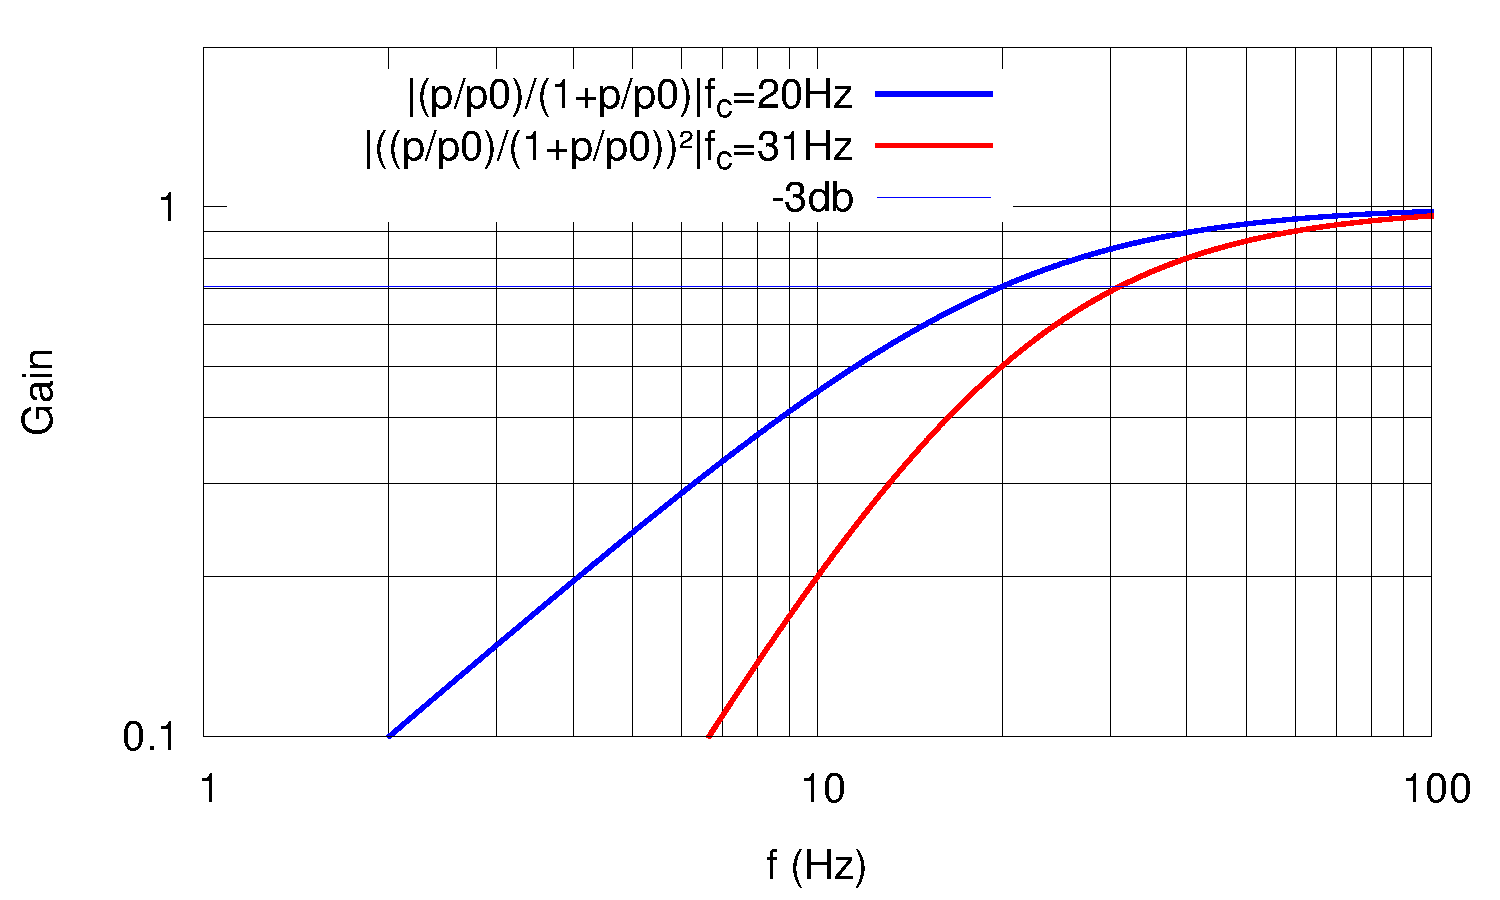
\includegraphics[width=10cm]{bode_corr_20-31.pdf}
\end{center}
%
L'étude théorique de la composition des filtres du premier ordre montre que la composée de $n$ filtres passe-haut du premier ordre ayant la \textbf{même} fréquence de coupure $f_c$ auront une fréquence de coupure qui vaudra\footnote{La démonstration de cette propriété est laissée au lecteur, il suffit d'exprimer la composée et identifier pour quelle fréquence son gain vaut $-3dB$.} $$f_{c_{\mbox{composée}}}=\frac{f_c}{\sqrt{2^{1/n}-1}}$$ Dans le cas présent, pour que la fréquence de coupure du système soit $f_{c_{\mbox{composée}}}=20Hz$, il faudra choisir $f_c=12.8Hz$.
%Les valeurs des dimensionnements qui corres

%Le dimensionnement fait pendant le labo considère des fréquences de coupures différentes à l'entrée et à la sortie. Les surdimensionnements dus à l'utilisation de valeurs normalisées permettent d'obtenir une fréquence de coupure de 20Hz.{\color{white}(mais c'est un peu par chance)}

%La réponse en fréquence des deux solutions se trouve sur le graphe suivant :
%\begin{center}
%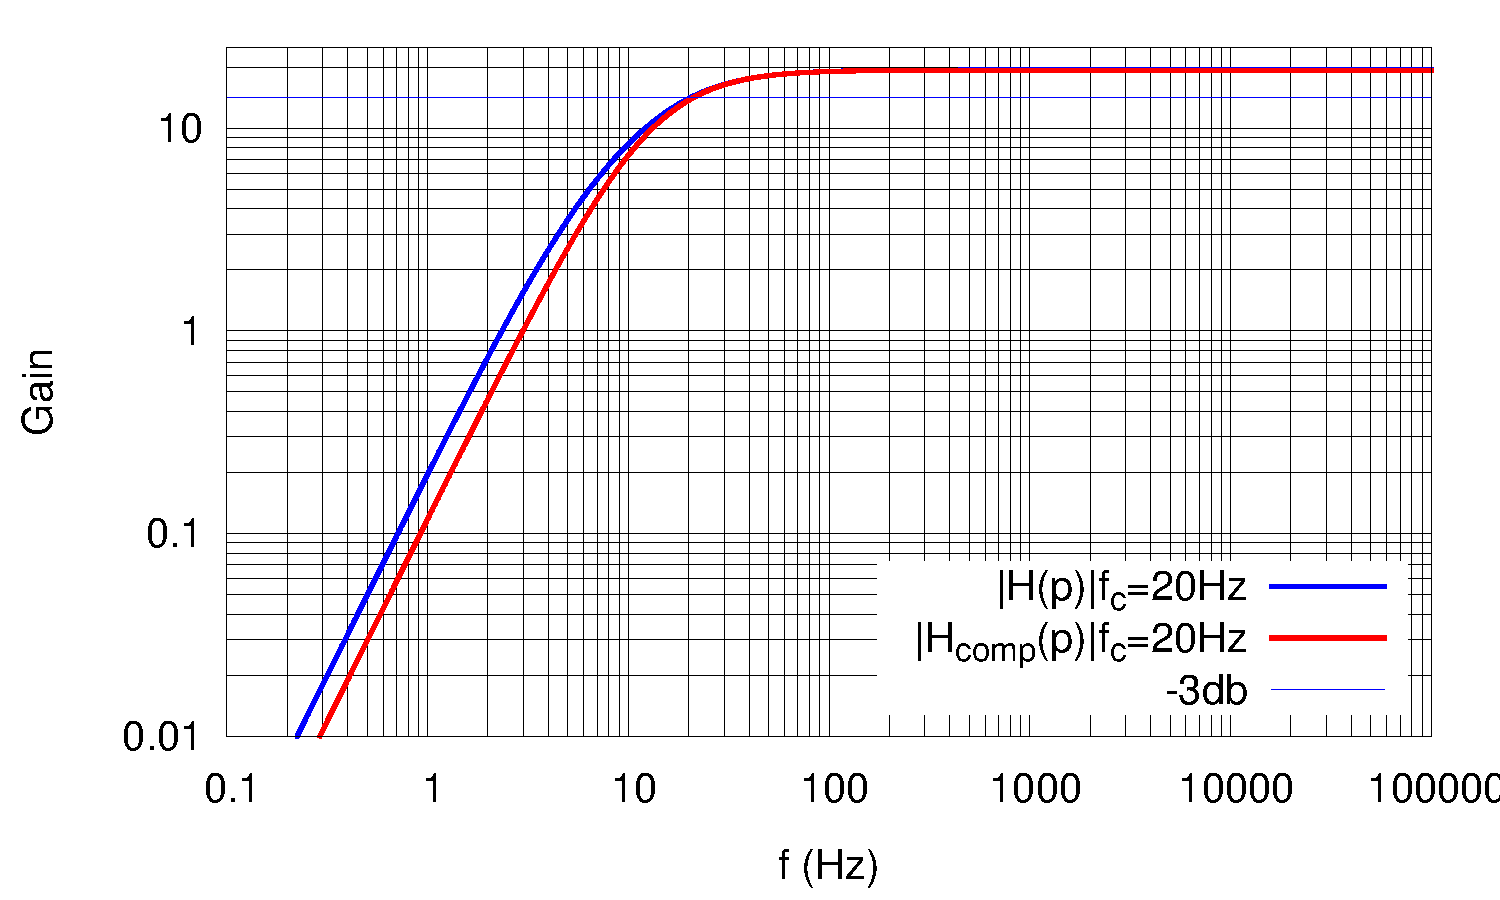
\includegraphics[width=10cm]{bode_corr.pdf}
%\end{center}

%Pour que ce corrigé soit cohérent avec la démonstration faite pendant le labo, la suite du dimensionnement sera effectuée en considérant $20Hz$ comme fréquence de coupure pour chaque filtre.

%Les valeurs correspondant à $f_c=12.8Hz$ sont toutefois précisées entre parenthèses dans la suite du document.

\subsubsection{Capacité d'entrée}
On désire amplifier un signal audio, par conséquent, l'entrée du circuit doit être un filtre passe-haut de fréquence de coupure inférieure à $20Hz$ à $-3dB$. Il faut également éviter que la composante continue appliquée sur la grille implique un courant continu dans la source de tension d'entrée.

Le schéma a petits signaux du montage fait apparaître que :
$$f_{c_{in}}=\frac{1}{2\pi\cdot\left(R_{b1}//R_{b2}\right)\cdot C_{in}}\leq 12.8Hz$$

En choisissant $R_{b1}=R_{b2}=100 k\Omega$, on trouve $C_{in}\geq 248nF$ la valeur normalisée la plus proche est $270nF$ qui donne une fréquence de coupure de $11.8Hz$ aux tolérances sur les composants près.

\begin{center}
\fbox{$R_{b1}=R_{b2}=100 k\Omega$}
\fbox{$C_{in}=270nF$}
\end{center}

%Avec $C_{in}=270nF$, on obtient $f_c=11.8Hz$.


\subsubsection{Capacité de sortie}
Il s'agit de couper la composante continue ajoutée pour pouvoir amplifier, une nouvelle fois, un filtre passe-haut est nécessaire.
La charge branchée sur cet étage est inconnue à priori, seule son impédance minimale est connue,  il s'agit du pire cas.

Le schéma à petit signaux et une transformée Norton--Thévenin fait apparaître que :

$$f_{c_{out}}=\frac{1}{2\pi\cdot\left(R_{D}+R_{ch}\right)\cdot C_{out}}\leq 12.8Hz$$ 

Dans le pire cas ($R_{ch}=3.3k\Omega$), $C_{out}\geq 3.6\mu F$, qui donnera la fréquence de coupure basse maximum du filtre. Si la charge a une impédance plus grande, la fréquence de coupure sera plus faible.

\begin{center}
\fbox{$C_{out}\geq 3.9\mu F$}
\end{center}

\subsubsection{Impédance de sortie}
Le même schéma à petit signal permet d'identifier l'impédance de sortie qui vaut : $$Z_{out}=R_D+\frac{1}{jC_{out}\omega}$$

Dans toute la bande passante, on veut $Z_{out}\leq 1k\Omega$, ce qui implique $$C_{out}\geq \frac{1}{2\pi\cdot f_c \sqrt{Z_{out_{lim}}^2-R_D^2}}$$

D'où $C_{out}\geq 8.0\mu F$.

Avec l'autre contrainte sur $C_{out}$, on peut choisir $C_{out}=8.2\mu F$ (valeur normalisée).

Ce qui permet d'avoir $f_{c_{out}}\leq 5.6Hz$ et respecter la contrainte sur l'impédance de sortie et sur la fréquence de coupure.

%\subsection{Consommation électrique}
%
%Il n'y avait pas de contrainte sur la consommation électrique, mais on peut 
%
%Le circuit consomme en moyenne :
%$$P_{circuit}=\frac{V_{dc}^2}{R_{b1}+R_{b2}}+E\cdot I_D$$%+{E\cdot i_{out}(R_{ch},t) }$$ avec $i_{out}=\frac{-A_v\cdot g_m \cdot v_{in}(t)}{R_{ch}}$
%
%La première contribution est négligeable devant l'autre avec les valeurs choisies.

\begin{center}
\fbox{$C_{out}= 8.2\mu F$}
\end{center}

\subsubsection{Bande passante totale du montage}

L'analyse de l'expression complète du gain en fonction de tous les éléments du circuit permet d'obtenir la fréquence de coupure à $-3dB$ du montage qui doit valoir $20Hz$ maximum. Comme il y a deux filtres, il est nécessaire de vérifier si la composée des deux respecte les contraintes, ce qui est le cas ici.

Si la bande passante n'avait pas été respectée, il aurait fallu diminuer la fréquence de coupure la plus élevée entre les deux filtres.


\subsection{Récapitulatif}

\begin{center}
\begin{tabular}{lll}
$E=12V$ & $R_D=150\Omega$ & $C_{in}=270nF$ \\ 
%\hline 
$V_{dc}=5.90V$ & $R_{b1}=R_{b2}=100 k\Omega$ & $f_{c_{in}}=11.8Hz$ \\ 
%\hline 
$V_{DS}=6.0V$ & $I_D=40mA$ & $C_{out}=8.2\mu F$ \\ 
%\hline 
$V_{GS}=2.95V$ & $f_{c_{\mbox{totale}}}=13.8Hz$ & $f_{c_{out}}=5.6Hz$ \\ 
\end{tabular} 

\end{center}

{\color{white}Je ferme ici la parenthèse laissée ouverte au labo \no 4 : )}

Le graphe des dépendances entre paramètres/contraintes est :

%\begin{tikzpicture} [>=spaced stealth’]
%\graph [layered layout, components go right top aligned, nodes=draw, edges=rounded corners]
%{
%first root -> {1 -> {2, 3, 7} -> {4, 5}, 6 }, 4 -- 5;
%second root -> x -> {a -> {u,v}, b, c -> d -> {w,z} };
%third root -> child -> grandchild -> youngster -> third root;
%};
%\end{tikzpicture}
\begin{tikzpicture}[->, >=latex,minimum size= 1.25cm,scale=0.9]
%\usetikzlibrary{arrows,decorations.markings}
%\def \n {5}
%\def \radius {3cm}
%\def \margin {8} % margin in angles, depends on the radius
\usetikzlibrary{calc}
%\usetikzlibrary{arrows.meta}
%\foreach \s in {1,...,\n}
{

%\tikzset{>={Latex[width=3mm,length=3mm]}}
%/pgf/;
  \node[draw, circle] (id) at (0-90:2) {$I_D$};
  \node[draw, circle] (vdsq) at (72-90:2) {$V_{DS}$};
  \node[draw, circle, color=red] (vout) at (144-90:2) {$v_{out}$};
   \node[draw, circle, color=red] (av) at (-144-90:2) {$A_{v}$};
    \node[draw, circle] (gm) at (-72-90:2) {$g_m$};
    
    
%    /pgf/arrow keys/length= 10mm;
  \draw   (id) to (vdsq);
  \draw (vdsq) -- (vout) ;
   \draw (vout) to (av);
   \draw(av) to (gm);
   \draw(gm) to (id);
  \draw (gm) to (av);
   \draw(av) to (vout);
 \draw  (id) to (gm);
 
 \coordinate (in) at ($(72-90:2)+(20:4)+(0.5,0)$){};
% (in)++(1,1);
  \node[draw, circle] (vdc) at (in) {$V_{dc}$};
  \node[draw, circle] (rb1) at ($(in)+(135:2) $) {$Rb_1$};
  \node[draw, circle] (rb2) at ($(in)+(-45:2) $) {$Rb_2$};
   \node[draw, circle, color=red] (zin) at ($(in)+(45:2) $) {$Z_{in}$};
   \node[draw, circle] (cin) at ($(in)+(45:4) $) {$C_{in}$};
   \node[draw, circle, color=red] (fcin) at ($(in)+(45:7) $) {$f_{C_{in}}$};
   
   \node[draw, circle] (vgsq) at ($(in)+(45:-2) $) {$V_{GS}$};
  
  \draw (id) to (vgsq);
  \draw (vgsq) to (id);
  \draw (vgsq) to (vdc);
  \draw (rb1) to (vdc);
  \draw (rb2) to (vdc);
  \draw (zin) to (rb1);
  \draw (zin) to (rb2);
  \draw (zin) to (cin);
  \draw (fcin) to (cin);
  \draw (fcin) to (rb1);
  \draw (fcin) to (rb2);
  
	\coordinate (out) at ($(av)+(105:2)$){};
% (in)++(1,1);
  \node[draw, circle, color=red] (zch) at ($(out)+(-30+15:2)$) {$Z_{ch}$};
  \node[draw, circle, color=red] (fcout) at ($(out)+(30+15:2)$) {$f_{c_{out}}$};
  \node[draw, circle] (cout) at ($(out)+(90+15:2)$) {$C_{out}$};
   \node[draw, circle, color=red] (zout) at ($(out)+(150+15:2)$) {$Z_{out}$};
   \node[draw, circle] (rd) at ($(out)+(210+15:2)$) {$R_{D}$};
%   \node[draw, circle] (fcin) at ($(out)+(-30:3)$) {$f_{C_{in}}$};
   
 %  \node[draw, circle] (vgsq) at ($(in)+(45:-2) $) {$V_{GSQ}$};
  
  \draw (av) to (rd);
  \draw (rd) to (fcout);
  \draw (zout) to (rd);
  \draw (zout) to (cout);
  \draw (fcout) to (cout);
  \draw (zch) to (fcout);
  \draw (zch) to (av);
  
  \draw (av) to (vgsq);
  
  \coordinate (pow) at ($(id)$){};
% (in)++(1,1);
  \node[draw, circle, color=red] (e) at ($(pow)+(-135:2)$) {$E$};
  \node[draw, circle, color=red] (pt) at ($(pow)+(-45:2)$) {$P_T$};
  \draw (e) to (id);
  \draw (pt) to (id);
  
  \node[draw, circle, color=red] (cont) at (-2,-6) {contrainte};
  \node[draw, circle] (param) at (6,-6) {paramètre};
  
	\node[draw, circle, color=red] (vin) at ($(vout)+(45:2)$) {$v_{in}$};  
	\draw (vin) to (vout);
  
  \draw (cont) to node [midway, above=-2mm] {influe sur/limite}(param);
%  \draw (zin) to (rb1);
%  \draw (zin) to (rb2);
%  \draw (zin) to (cin);
%  \draw (fcin) to (cin);
%  \draw (fcin) to (rb1);
%  \draw (fcin) to (rb2);  
  
  % ({360/\n * (\s - 1)+\margin}:\radius) 
   % arc ({360/\n * (\s - 1)+\margin}:{360/\n * (\s)-\margin}:\radius);
}
\end{tikzpicture}

\newpage
\begin{center}
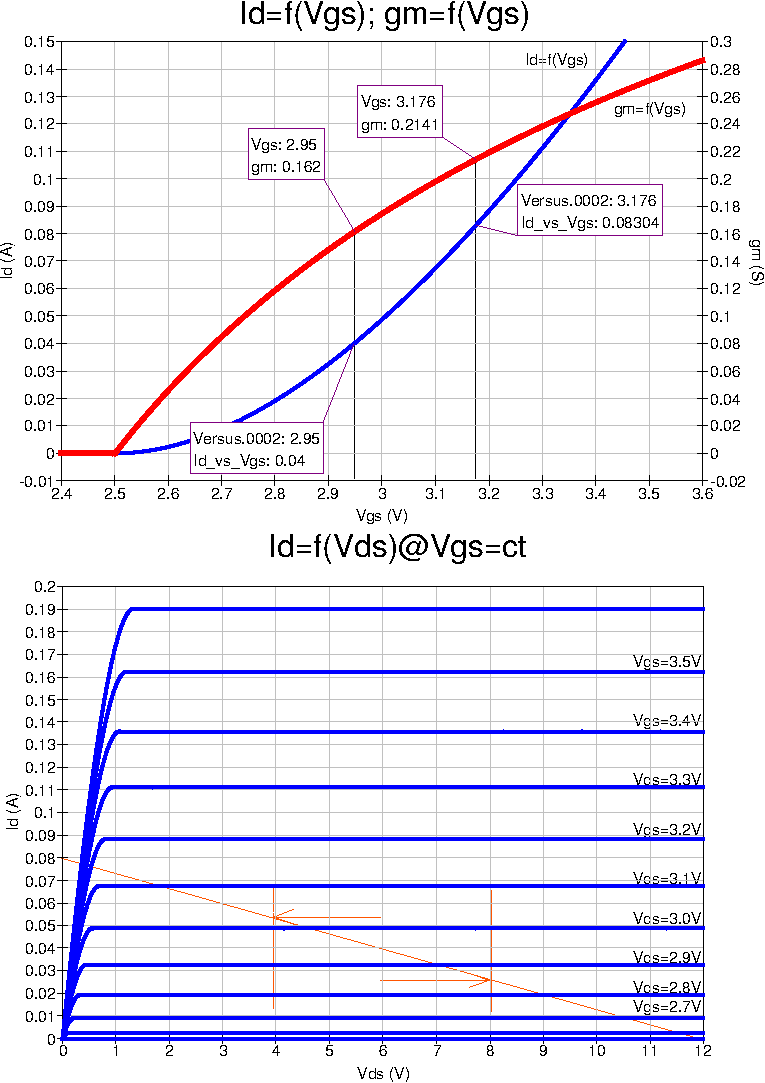
\includegraphics[width=15cm]{courbes_mos_2k16-crop_corr.pdf}
\end{center}
}%réponse
\ifthenelse{\not \boolean{annexes}}{\end{document}}{}
\clearpage
\appendix
\newgeometry{top=1 in, bottom=1 in, left=1 in, right=1 in} % Yeah, that's bad to play with margins


\end{document}